\documentclass[twoside,12pt]{book}

\def\mytitle{Graphs and Information Retrieval}
\def\myauthor{Chris Kamphuis}
\def\mydate{\formatdate{22}{03}{2023}}

\usepackage[utf8]{inputenc} % Input encoding
\usepackage[T2A,T1]{fontenc}    % Font encoding
\usepackage{lmodern}        % Nicer font
\usepackage{microtype}      % Better kerning
\usepackage{tipa}           % IPA symbols
\usepackage{stmaryrd}       % short arrows
\usepackage{textcomp}       % upquote
\usepackage{titlecaps}      % titlecase commands
\usepackage{amsmath}        % extra math
\usepackage{amssymb}        % extra math symbols
\usepackage{relsize}        % \smaller command
\usepackage{siunitx}        % typeset units
\usepackage{xcolor} 

\definecolor{ruhuisstijlrood}{rgb}{0.745,0.192,0.102}

\usepackage{geometry}
\geometry{
	inner=25mm,
	outer=20mm,
	marginparsep=3mm,
	marginparwidth=13mm,
	top=25mm,
	bottom=20mm,
	paperwidth=17cm,
	paperheight=24cm,
}
%graphics
\usepackage{graphicx}
\usepackage{pdflscape}
\usepackage{float}
\usepackage{fancyhdr}
\usepackage{caption}  % subfigures
\usepackage{subcaption}
\usepackage{rotating}
% Tables
\usepackage{booktabs}  % Nicer tables
\usepackage{multirow}  % Multirow cells
\usepackage{tabularx}  % Automatically wrapping tables
\usepackage{longtable} % Tables spanning pages
\usepackage{threeparttable} % Tables with footnotes
% todo set listings for SQL and GQL
\usepackage{listings}

\usepackage{bookmark}
\usepackage[noabbrev]{cleveref} % Easy references
\usepackage{xr}
\usepackage{subfiles}


\usepackage{todonotes}
\setuptodonotes{
	backgroundcolor=white,
	linecolor=black,
	size=tiny,
}

\author{\myauthor}
\title{\mytitle}
\date{\mydate}

\begin{document}

\frontmatter

\begin{titlepage}
	\begin{center}
		\vspace*{3.5cm}
		
		%		\LARGE{\textsc{\bfseries\mytitle}}
		\huge{\bfseries\mytitle}
		
		\vspace*{15pt}
		
		%		\large{\textsc{\mysubtitle}}
		% \Large{\mysubtitle}
		
		\vspace*{5pt}
		
		%	    \large{\textsc{More subtitle}}
		\normalsize
		
		\vspace{2.0cm}
		
		\textbf{Proefschrift}
		
		\vspace{0.5cm}
		
		ter verkrijging van de graad van doctor\\
		aan de Radboud Universiteit Nijmegen\\
		op gezag van de rector magnificus
		prof.~dr.~J.M.\ Sanders,\\
		volgens besluit van het college van decanen\\
		in het openbaar te verdedigen
		
		\vspace{0.5cm}
		
		op woensdag -- -- 2025\\
		\vspace{0.2cm}
		om 12:00 uur precies
		
		\vspace{0.5cm}
		
		door
		
		\vspace{0.5cm}
		
		\textbf{\myauthor}\\
		
		geboren op 22 maart 1993\\
		te Oldenzaal, Nederland
	\end{center}
\end{titlepage}

\newpage%

\thispagestyle{empty}

\begin{itemize}
	\item[] Promotor:
	\begin{itemize}
		\item[] prof.\ dr.\ ir.\ A.P.\ (Arjen)\ de\ Vries
	\end{itemize}
\end{itemize}

\begin{itemize}
	\item[] Manuscriptcommissie:
	\begin{itemize}
		\item[] \makebox[4.2cm]{Person A\hfill} (Affiliation)
		\item[] \makebox[4.2cm]{Person B\hfill} (Affiliation)
		\item[] \makebox[4.2cm]{Person C\hfill} (Affiliation)
		\item[] \makebox[4.2cm]{Person D\hfill} (Affiliation)
		\item[] \makebox[4.2cm]{Person E\hfill} (Affiliation)
	\end{itemize}
\end{itemize}

\vfill

\noindent%
%\begin{minipage}[b][][b]{0.8\textwidth} % adapt widths of minipages to your needs
\begin{minipage}[b][][b]{0.95\textwidth} % adapt widths of minipages to your needs
	{
		\setlength{\parindent}{0cm}%
		This work is part of the research program Commit2Data with project number 628.011.001 (SQIREL-GRAPHS), which is (partly) financed by the Netherlands Organisation for Scientific Research (NWO).
		
	}
	
	\vspace{0.25cm}
	
	{
		\setlength{\parindent}{0cm}%
		Printed by a drukkerij met een naam\\[\baselineskip]
		Typeset using \LaTeX\\[\baselineskip]
		ISBN:\ 111{-}11{-}11111{-}11{-}1\\[\baselineskip]
		Copyright \copyright{} Chris Kamphuis, 2025\\[\baselineskip]
	}
\end{minipage}%
%\hypersetup{pageanchor=true}
\tableofcontents

\mainmatter
\chapter{Introduction}
\label{chp:introduction}
\epigraph{I \textit{propose} to consider the question, ``Can machines think?''}{Alan Turing - 1950}

I also propose to consider the question, ``Can machines think?'' Instead of approaching this through a thought experiment as Turing did, nowadays, one can approach this question by asking it to a search engine. When issuing this query to popular web search systems, we get varying results: the first result on Google is a passage generated from the article written by Turing, while the first result on Bing is a passage generated from a website that concludes machines cannot think\footnote{However, if a machine cannot think, can we trust the result presented by this algorithm?}\footnote{These results were retrieved in October of 2022}.

We use systems that process queries daily when looking for \textit{information}. While Google and Bing are all-purpose web engines that mainly focus on finding and retrieving information from the internet, people also use specialized search systems in their day-to-day lives: Amazon and eBay when we are looking for a product to buy, Scholar and ResearchGate for scientific resources, Youtube and TikTok for Videos, or Facebook and LinkedIn when we are searching for people. It might even be possible that you are reading this text after you found this document through search. 

When searching for the query, ``Can machines think?'', searching through text documents might be sufficient for the person who searches. However, more than only considering text is needed when someone's information need is more complicated. For example, when one wants to buy a product on Amazon, aspects other than text also need to be considered. Maybe you want to buy an iPhone; information on the price, which edition is the most recent, or which color it has are all essential to determine which one you want. You may also want to consider the rating provided by people that previously bought an iPhone.

If someone searches for people on LinkedIn, they are generally more interested in persons they are connected to than strangers. If you are looking for someone to do a job, it is ideal that a shared connection can vouch for them. In this case, how people relate to each other in their network might indicate \textit{relevance}. Not only the structure of how people relate to each other determines relevance; their experience, where they work, or reviews of their previous work might also matter.

Although it might be possible to encode all this information as written text, often, it is more convenient to save this information in a more structured approach. Where information retrieval researchers research the retrieval of ``information'' through text data, data management researchers research the retrieval of structured data. This thesis considers both methods simultaneously: systems that can work with structured and unstructured information are investigated.

\section{Problem Description and Research Questions}
Although information retrieval and data retrieval are research fields investigated by different disciplines, they are closely related, and systems that use both have been researched and developed in the past. Techniques developed in one community might help the other, as things like storing and quickly retrieving data are essential for information and data retrieval. 

In recent years there has been much exciting research in the database community studying graph databases. As these databases are becoming more popular for data retrieval tasks where the data is highly interconnected, they might also benefit similar tasks in the information retrieval field where data is often highly interconnected. This thesis will investigate how these databases, with dedicated graph query languages, can be used for information retrieval tasks. This leads us to this thesis's main research question: \textbf{Research Question: How can information retrieval benefit from graph databases and graph query languages?}

Three sub-research questions are defined to guide us in answering the main research question:

\begin{enumerate}
	\item \emph{Research Question 1: What are the benefits of using relational databases for information retrieval?} 
	\item \emph{Research Question 2: Can we extend the benefits from using relational databases for information retrieval to using graph databases while being able to express graph-related problems easier?} 
	\item \emph{Research Question 3: When does information retrieval research benefit from graph data?} 
\end{enumerate}

\cref{ir-using-relational-databases,from-tables-to-graphs,ch:mmead} will take these research questions and try to answer them. Then in~\cref{conclusion}, we will try to take the answers to these questions and use them to answer the main research question. 

\section{Thesis Contributions and Structure}

\begin{itemize}
	\item Chapter~\ref{related-work} will describe all necessary background information to provide context to the other chapters. The background that is described in this chapter concerns the ``general'' background knowledge for this thesis. Individual chapters will also have related work sections that concern the background knowledge in those chapters. The information described in those related work sections might contain overlapping information, i.e., the knowledge needed to understand the context of those chapters. This is done to make it possible to understand a chapter without first reading the chapters that come before it. 
	
	\item Chapter~\ref{ir-using-relational-databases} concerns information retrieval research using relational databases. 
	Although, traditionally, inverted indexes are used for information retrieval, we show that by employing relational databases, some advantages are gained. 
	First, attempts to use relational databases for information retrieval through the years will be described. One of the latter attempts used a column-oriented relational database system for information retrieval, achieving competitive efficiency compared to a traditional system built using inverted indexes. This approach is re-implemented as a prototype system used, which is then used for a reproduction study. This chapter establishes the usefulness of relational databases for information retrieval by demonstrating its benefits. The content in this chapter is based on the following published works: 
	
	{
		\scriptsize
		\begin{itemize}
			\item \bibentry{olddog-docker}
			\item \bibentry{Kamphuis2020BM25}
		\end{itemize}
	}
	
	\item Chapter~\ref{from-tables-to-graphs} takes the concept of employing relational databases for information retrieval and extends the relational model to the graph model. GeeseDB is introduced, a graph database prototype system built on top of an embedded column-oriented relational engine. Using the graph model makes it possible to express more complex information retrieval problems than when the relational model is used. These more complex models often use multi-stage retrieval approaches. GeeseDB is built on top of an embedded database system, so moving data between ranking stages can be done efficiently. The content of this chapter has previously been described in the following published works:
	
	{
		\scriptsize
		\begin{itemize}
			\item \bibentry{need-graph-db}
			\item \bibentry{geesedb}
		\end{itemize}
	}
	
	\item Chapter~\ref{a-graph-of-entities} introduces the concept of entity linking. Specifically, the Radboud Entity Linker~\citep{rel} system is discussed. When trying to utilize REL to annotate a large corpus with entity linking, issues were found that prohibited the annotations process to such an extent that it was not possible to do within a reasonable time. In order to be able to annotate the corpus, the REL toolkit internals were upgraded, and a batch extension was developed. Altogether this led to more efficient software such that REL can annotate larger corpora. The content in this chapter has previously been described in the following published work: 
	
	{
		\scriptsize
		\begin{itemize}
			\item \bibentry{rebl}
		\end{itemize}
	}
	
	\item Chapter~\ref{ch:mmead} will employ the software described in the chapter before it and uses it to annotate a large web corpus. We developed a specification of how entity link annotations can be shared for these annotations. Following this specification, we made the annotations for the MS MARCO~\citep{msmarco} corpora publicly available. Using these annotations, we show that, through query expansion, we can increase recall effectiveness for first-stage rankers on this dataset. Next, a demonstration shows how entity links can also be used for geographical information applications. 
	This content has been described in the following work, accepted for publication; 
	
	{
		\scriptsize
		\begin{itemize}
			\item \bibentry{mmead}
		\end{itemize}
	}
	
	\item Chapter~\ref{conclusion} will serve as a conclusion and tries to summarize the content discussed in the book. Here we will reflect on the research question and discuss what future research is needed.
\end{itemize}

\section{Other Publications}
During the employment at Radboud University, the following work was also published: 

{\scriptsize
	\begin{itemize}	
		\item \bibentry{trec-2019}
		\item \bibentry{ciff}	
		\item \bibentry{trec-2020}
		\item \bibentry{trec-covid}
		\item \bibentry{graphdb-for-ir}
	\end{itemize}
}

Although this work relates to the main subject of the thesis, it is not used as source material for the work described in this thesis. 
\chapter{IR using Relational Databases}
\section{Introduction}
Where commonly information retrieval researchers use inverted indexes as data structures, there is also a rich history of researchers using relational databases for representing the data in information retrieval systems. 

% Describe boolean retrieval systems
% Describe other systems by for example Norbert 

In a more recent work \cite{OldDog} showed that the common used BM25 ranking function can also be easily expressed using relational tables. Their work specifically focused on the retrieval efficiency of several systems.   
% End with OldDog system by Hannes

\section{Reproducibility}

We \cite{Kamphuis2020BM25}
\chapter{From Tables to Graphs}
\label{from-tables-to-graphs}
\epigraph{``The reader will have anticipated that I have no very convincing
	arguments of a positive nature to support my views. If I had I should not
	have taken such pains to point out the fallacies in contrary views.``}{Alan Turing - 1950}

\begin{Abstract}
	\begin{changemargin}{1cm}{1cm}
		This chapter introduces GeeseDB. GeeseDB is a Python toolkit for solving information retrieval research problems, that leverages graphs as data structures. It aims to simplify information retrieval research by allowing researchers to formulate graph queries through a graph query language. GeeseDB is built on top of DuckDB, an embedded column-store relational database for analytical workloads. GeeseDB is available as an easy-to-install Python package. In only a few lines of code, users can create a first-stage retrieval ranking using BM25. Queries read and write Numpy arrays and Pandas dataframes at negligible data transformation cost. Therefore, the results of a first-stage ranker expressed in GeeseDB can be used in various stages in the ranking process, enabling all the power of Python machine learning libraries with minimal overhead.
	\end{changemargin}
\end{Abstract}

\section{Introduction}
In recent years there has been a lot of exciting new information retrieval research that uses non-text data to improve the efficacy of search applications. All these research directions have improved search systems' effectiveness by using more diverse data. Although more diverse data sources are considered, these systems are often implemented through a coupled architecture. In particular, first-stage retrieval is often carried out with different software than that used in later retrieval stages, where these novel reranking techniques tend to be used. In our view, researchers could benefit from a system where retrieval stages are more tightly coupled, which facilitates the exploration of how to use non-content data for ranking and serves the data in a format suitable for reranking with, e.g., transformers, tree-based methods or graph-based methods.

The previous chapter demonstrates how relational databases can be used for information retrieval problems. Integrating alternative data sources into search systems is easier when using a relational database instead of an inverted index. In the case of information retrieval, graph data can often be used to improve search effectiveness. One of the most famous examples where graphs help information retrieval is the PageRank algorithm~\citep{pagerank}. Although it might be possible to express ranking over graph data in relational databases, they are not designed with graph structures in mind. 

The data management community has shown much interest in graph databases in recent years. Graph databases are different from relational databases in that graphs are the main representation for managing the data, instead of the usual relations. Graphs can be considered a better abstraction for real-world data than relations. Graphs focus much more on concepts (nodes in a graph) and how they relate to each other (edges in a graph), while in a relational database this information is implicit, requiring knowledge of the schema. From the types of graphs discussed in \cref{related-work}, we focus on using \emph{property graphs} in this chapter. This type of graph contains nodes and directed edges, which can be labeled; nodes and edges can also have associated key-value pairs.

The research goal in this chapter is two-fold; firstly, we develop a system that can search efficiently in information represented as graphs. In the previous chapter, we showed that relational databases could search efficiently and help reproducible research. However, these systems do not support graph data structures directly in their interface to the user (e.g., the query language). Systems built on inverted indexes use coupled architectures, which can introduce unnecessary overhead.

Secondly, we want to create a system where both first and second-stage retrieval are directly supported. In IR research, multi-stage retrieval systems contain components that are not run in the same ecosystem; introducing overhead in retrieval efficiency. 
So in this chapter, the prototype system GeeseDB is introduced; it tries to leverage the same techniques for search as relational databases do while also naturally being able to support graphs. This leads to the main research question for this chapter:

\begin{itemize}
	\item[\textbf{RQ2:}] Can we extend the benefits from using relational databases for information retrieval to using graph-databases while being able to express graph-related problems easier?
\end{itemize} 

In order to answer this research question, we will use our own prototype system GeeseDB. Before introducing GeeseDB, we first look into work that uses systems that combine two systems for two-stage retrieval experiments, and systems built for processing graphs.

% rewrite and reflect on the previous chapter, and give context in which graph databases are helpful.

\section{Related work }
% Describe the related work which was presented in the GeeseDB paper, but also include more related work regarding approaches that use graph language-like approaches (different subsection). 
In modern IR it is not uncommon to use coupled architectures. In many situations a ranking model is used that is efficient, but only reasonably effective. BM25 can be considered a model that can be calculated cheaply providing a good score for a more advanced (but less efficient) retrieval model that could achieve higher effectiveness. In such cases, BM25 can be used to calculate an initial top-$k$ ranking that contains (presumably) all relevant documents. Then, the more expensive model only has to calculate the final ranking scores over the top-$k$ documents.

In this section we start discussing methods that implement multi-stage approaches, then systems that implement them are highlighted. In particular there will be a focus on the coupled-architectures aspect of these systems. Finally, some proposed methods will be discussed to deal with cons arising from coupled architectures. 

\subsection{Learning To Rank}
In learning-to-rank (LTR), multi-stage retrieval approaches are widely used; LTR models are not efficient enough to compute a relevance score value for all documents in the collection.
In these cases, a decision tree based ensemble like LambdaMART~\citep{lambdamart} tends to be trained. These models take input that is usually not stored in an inverted index. So, in order to use these models, the output from the inverted index needs to be combined with other data.

\Citet{ltr-1} showed that for the TREC Contextual Suggestion track~\citep{contextual-suggestion-track}, reranking using user-based features significantly improved retrieval effectiveness over a baseline language modeling approach. These features show that data not present in the document's text can help the retrieval effectiveness of systems; metadata helps to rank. 

\Citet{ltr-2} show examples of features that have been effective for learning to rank, many of these features are non-textual. Some influential features are: click count, click entropy, and the number of displayed results in a session. 

\subsection{Dense Retrieval}
Where traditionally, search was carried out using inverted indexes, neural retrieval has become more prevalent in recent years. When neural retrieval \citep{neural-ir} is implemented as a vector search approach, it is referred to as dense retrieval.
Consider, for example, the work by \citet{dense-retrieval-1}; in their work, they proposed \texttt{clear}, a model that aims to complement lexical models with a dense retrieval model. In their study, they use BM25 as the lexical model. The BM25 scores are calculated using an inverted index (Anserini~\citep{anserini}), while the dense retrieval model is a fine-tuned BERT bi-encoder. This dense model calculates a score using a different maximum inner-product search (MIPS) system (Faiss~\citep{faiss}) to calculate a similarity score for the query document pairs. Then scores are weighted and summed to calculate a new ranking score value. 

In a similar study, \citet{dense-retrieval-2} compared several methods on the MS Marco document and passage datasets. In their work, one of the two best models on the passage dataset was to combine a lexical model with a BERT-based bi-encoder. The scores were combined by retrieving the top-\textit{n} documents for both the lexical model and the bi-encoder. In order to do this, an inverted index (Anserini) is used to retrieve the documents for the lexical model, while the bi-encoder uses a MIPS system (ScaNN~\citep{scann}).

A third example, is the study of  \citet{dense-retrieval-3} that experiments with distilled dense representations. They do an extensive comparison study, and in their work, the best results are reported by either multi-stage or hybrid dense + sparse retrieval methods. The multi-stage retrieval method used BM25 in combination with BERT-large. Although effective, it is a method with a high latency because of the cross-encoder used. A TCT-ColBERT (Tightly-Coupled Teacher - ColBERT) bi-encoder with doc2query-T5 sparse retrieval was the best hybrid method. This sparse retrieval method is a BM25 retrieval method that expands the documents with T5 language model questions~\citep{2020t5}. These questions were generated by letting the T5 language model generate questions that the passage might answer. Sparse retrieval is carried out by Anserini, and dense retrieval by Faiss. 

\subsection{Knowledge Graphs and Entities}
% knowledge graphs to leverage entity information~\cite{entity-1, entity-2, entity-3}, 
Knowledge graphs have been used a lot as well in IR research. \Citet{entity-1} proposed the Entity Linking incorporated Retrieval (ELR) approach. The idea behind this concept is that when entity annotations are available for queries and documents, they can be incorporated into the ranking model. Their publication only focuses on entity retrieval, but the method can generalize to ad-hoc document and passage retrieval. The entities are incorporated by creating a dedicated index for entities on which entity scores can be calculated. These are then merged by the document scores calculated using the regular index. By incorporating entity scores, ELR has been shown to increase effectiveness scores for multiple baseline methods. 

\Citet{entity-3} also used entity features for query expansion. One of the features was calculated by tagging queries with an entity-linking system. When entities were found, information from the knowledge base linked to them was included in query expansion. Alternative names of the entity were also included in the query expansion. Then, this expanded query provided a score for all documents. Another feature they calculate is obtained by ranking the entities in the knowledge base using the original query text. Then the data (e.g., words in the descriptions) included in the knowledge base can be included as terms for query expansion. Multiple other features using entities were also calculated, 

For additional background related to entities in search, refer to \Citet{entity-2}, an excellent book on entity-oriented search, that surveys many methods that use entities for search. 

Basically, in order to include entities, a knowledge graph needs to be queried. This tends to be done by a different systems than the systems used for regular retrieval. If we could integrate IR in graph databases, a single system would solve the complete process.
% maybe include a subsection about graphs including the work by mcdonald

\subsection{Current approaches}
Recently, retrieval methods using neural networks have become state-of-the-art, mainly using large language models. In this section the two most commonly used research systems are described, highlighting how they with neural approaches to IR.
PyTerrier~\citep{pyterrier} and Pyserini~\citep{pyserini} are modern research systems that are widely used for information retrieval research. These systems are built as inverted index systems, with a separate component to handle neural retrieval models. 

\subsubsection{PyTerrier}
PyTerrier by~\citet{pyterrier}, is a Python extension of Terrier~\citep{terrier}. Terrier is an open-source search engine system written in Java. It implements state-of-the-art indexing and retrieval techniques on top of an inverted index. It is a system suited for rapidly developing retrieval experiments concerning document collections with many documents. 
The PyTerrier extension was developed to express complex IR pipelines in Python. Using Python operators directly, it is possible to set up an IR pipeline using PyTerrier in only a few lines of code. 

PyTerrier was expanded to support state-of-the-art large language model reranking approaches and dense retrieval methods. As the PyTerrier framework is developed for the Python ecosystem, other (re-)ranking methods that are implemented in Python can readily work with PyTerrier. The PyTerrier system is ideal for modern information retrieval research, that often concerns reranking through learned methods, as they are often developed in Python.

Note, however, that PyTerrier uses a coupled architecture. First-stage retrieval is carried out using Terrier in Java (e.g., a BM25 run), and then the resulting top documents are reranked in Python. For this, some overhead is introduced because of data transfer between processes. 

\subsubsection{Pyserini}
Pyserini was developed by~\citet{pyserini}, which is a Python extension of Anserini~\citep{anserini}. Pyserini and Anserini have a lot in common with PyTerrier and Terrier. Just like Terrier, Anserini is developed in Java, but on top of Apache Lucene. Anserini is developed as a system with solid support for reproducible research. Anserini provides reproducible baselines for many retrieval benchmarks that can be run with minimal investment of resources. 

Pyserini is developed as a Python wrapper around the Anserini retrieval system. Within the Python ecosystem, it is possible to access the Anserini internals and replicate the same experiments implemented in Anserini. Similarly to PyTerrier, Pyserini also contains features that are not available directly in Anserini; ranking methods that make use of large language models, such as dense retrievers and BERT-based cross encoders. As these methods are generally developed in Python, it is much easier to support them with Pyserini compared to Anserini.

Anserini is included in Pyserini as a JAR file, so when using Pyserini for first-stage retrieval, data needs to be retrieved from JAVA before it can be materialized in Python. The setup is similar to that of Pyterrier. 

\subsection{Proposed approaches}
% Paper van Jimmy op DESIRES is belangrijk. 
\subsubsection{Separation of the Logical and Physical Model}
% todo different compontent systems?? ask Arjen what it says?
As shown in the previous sections, dense and sparse retrieval methods are often implemented using different  systems, which  introduces the coupled architecture. \citet{seperation-logical-physical} recognizes that sparse retrieval models tend to be implemented using inverted indexes and dense retrieval methods with approximate nearest neighbor systems. Although these systems are different, the input and the output are the same: the input is a query, and the output is a ranked list of the top-$k$ documents the ranking methods deem the most relevant. 

In order to be able to formalize these similarities and distinctions more clearly, \citeauthor{seperation-logical-physical} proposes a distinction between the logical and physical retrieval models. Logical models specify encoders that map documents and queries to a representation, and a comparison function that defines how a ranking score value can be computed from comparing these representations. Physical models define how to create a top-$k$ ranking from a large corpus given a query. The most straightforward physical approach would simply apply the logical model to every query-document pair, but through optimizations it might not necessary to compare all documents to the query. For example, dense retrieval methods often make use of the HNSW datastructure for nearest neighbor search~\citep{faiss} which prunes documents that have a low likelihood of being relevant. 

\subsubsection{A Graph Query Language for IR}
% Reproducible IR needs a graph query language ook belangrijk
It would be ideal for a system to encapture these different ways of approaching IR research natively; work with multiple stages in the ranking process, but also reason about entities and knowledge graphs. 
\citet{need-graph-db} proposed to use a graph query language for information retrieval problems. In the context of separating logical and physical models, a graph query language can be interpreted as a logical model, while the engine that implements the graph query language can be considered the physical model.

If it is possible to express both first stage and second stage retrieval in such a query language, both stages would be computed by the same physical model, automatically ensuring a coupled architecture is not necessary. Having a graph query language available, ensures that more complicated retrieval strategies can be expressed compared to when a relational query language is used. 

So ideally we develop a system with the following two capabilities; the system supports first retrieval stage directly, and graph queries over the output of this first stage retrieval can be processed without a coupled architecture. In order to fulfill these needs, we developed GeeseDB in a follow up study. 

\section{GeeseDB}
% Introduce GeeseDB, and the approach of what we are doing with GeeseDB
GeeseDB\footnote{\url{https://github.com/informagi/geesedb}, last accessed January 22th 2024} is a prototype Python toolkit for information retrieval that leverages graphs as data structures, allowing metadata and graph-oriented data to be easily included in the ranking pipeline. The toolkit is designed to quickly set up first-stage retrieval and make it easy for researchers to explore new ranking models. 

In short, GeeseDB aims to provide the following functionalities:
\begin{itemize}
	\item GeeseDB is an easy-to-install, self-contained Python package available through \texttt{PyPI} with as few as possible dependencies. It contains topics and relevance judgments for several standard IR collections out-of-the-box, allowing researchers to develop new ranking models quickly. 
	\item First stage (sparse) retrieval is directly supported. In only a few lines of code, it is possible to load documents and create BM25 rankings. 
	\item Data is served in a usable format for later retrieval stages. GeeseDB allows directly running queries on Pandas data frames for efficient data transfer to sequential reranking algorithms.
	\item Easy data exploration is supported through querying data with SQL, but more interestingly, using a graph query language (based on the Cypher query language), making exploring new research avenues easier. This prototype supports a subset of the graph query language Cypher, similar to the property graph database model query language as described by~\citet{angles2018property}.
\end{itemize}

\section{Design}
% Expand the Design part a lot, how did we solve certain technical problems. 
At the core of GeeseDB lies the full-text search design presented by~\citet{OldDog} as discussed already in~\cref{ir-using-relational-databases}. This work proposes a column-store database for IR prototyping, which uses the database schema described in~\cref{olddog_schema}, consisting of three database tables.
\begin{figure}
	\centering
	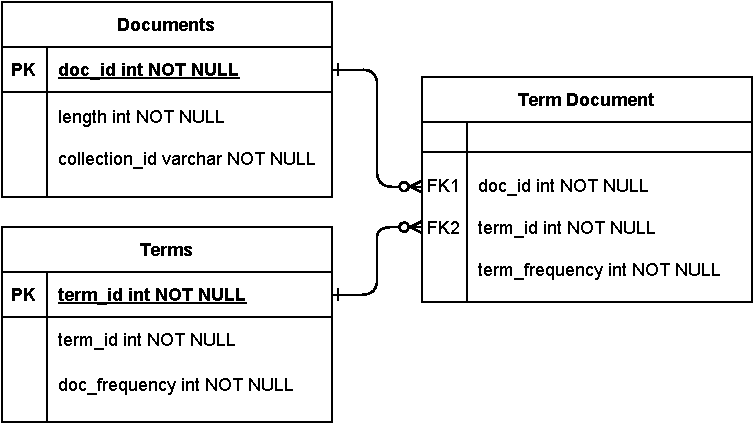
\includegraphics[width=\linewidth]{./imgs/olddog-schema-2.pdf}
	\caption{Database schema by \citeauthor{OldDog} for full text search in relational databases}
	\label{olddog_schema}
\end{figure}
Using these three tables, the authors show that BM25 can be easily expressed as a SQL query with latencies on par with custom-built IR engines. In GeeseDB, we use the same relational schema for full-text search.
Instead of seeing the document data and term data as tables that relate to each other through a many-to-many join table, it is also possible to consider this schema as a bipartite graph. In this graph, documents and terms are considered nodes connected through edges. If a term occurs in a document, an edge exists between that term and the document. GeeseDB uses the data model of property graphs labeled multigraphs where both edges and nodes can have property-value pairs. The database schema, as described in~\cref{olddog_schema}, would then translate to the property graph schema shown in~\cref{olddog-graph-schema}.
\begin{figure}
	\centering
	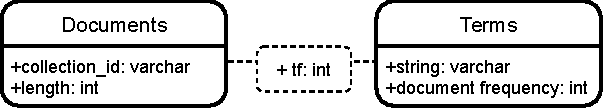
\includegraphics[width=\linewidth]{./imgs/olddog-graph-schema.pdf}
	\caption{Graph schema representing bipartite document-term graph}
	\label{olddog-graph-schema}
\end{figure}
A small example of a graph represented by this schema is shown in~\cref{example-olddog-graph}. Document nodes contain document-specific information (i.e., document length and the collection identifier), term nodes contain information relevant to the term (i.e., the term string and the term's document frequency), and the edges between document and term nodes contain term frequency information (i.e., how often is the term mentioned in the document represented the respective nodes it connects).
%\begin{figure}
%	\centering
%	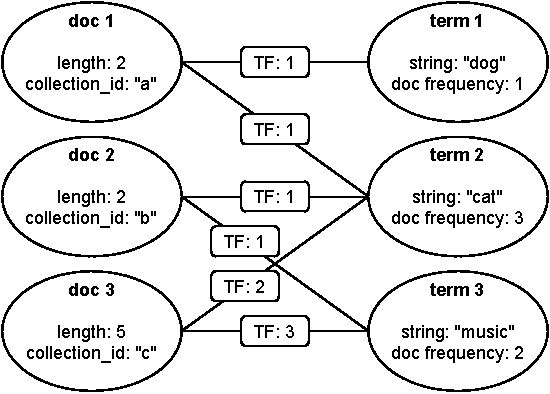
\includegraphics[width=\linewidth]{./imgs/example_olddog_graph.pdf}
%	\caption{Example term-document graph that maps to relational database schema}
%	\label{example-olddog-graph}
%\end{figure}

\begin{figure}
	\centering
	\begin{tikzpicture}[thick, node distance = {60mm}, main/.style = {draw, ellipse}] 
		\node[main, align=center, shape=ellipse] (1) {\underline{doc 1} \\ \textit{collection id:} "a" \\ \textit{len:} 2}; 
		\node[main, align=center] (2) [right of=1] {\underline{term 1} 
		\\ \textit{doc frequency:} 1 \\ \textit{string:} "dog"};
		
		\node[main, align=center, shape=ellipse, node distance=25mm] (3) [below of=1] {\underline{doc 2} \\ \textit{collection id:} "b" \\ \textit{len:} 2}; 
		\node[main, align=center, node distance=25mm] (4) [below of=2] {\underline{term 2} \\ \textit{doc frequency:} 2 \\ \textit{string:} "cat"};
		
		\node[main, align=center, shape=ellipse, node distance=25mm] (5) [below of=3] {\underline{doc 3} \\ \textit{collection id:} "c" \\ \textit{len:} 2}; 
		\node[main, align=center, node distance=25mm] (6) [below of=4] {\underline{term 3} \\ \textit{doc frequency:} 5 \\ \textit{string:} "music"};
		
		\draw (1) edge[align=center, bend left=10] node[above] {\textit{TF:} 1} (2);
		\draw (1) edge[align=center] node[yshift=1mm, above] {\textit{TF:} 1} (4);
		\draw (3) edge[align=center, bend left=10] node[above] {\textit{TF:} 1} (4);
		\draw (3) edge[align=center, bend left=20] node[yshift=-1mm, left] {\textit{TF:} 1} (6);
		\draw (5) edge[align=center, bend right=20] node[yshift=1mm, left] {\textit{TF:} 2} (4);
		\draw (5) edge[align=center, bend right=10] node[below] {\textit{TF:} 3} (6);
		
		
	\end{tikzpicture}
	\caption{Example term-document graph that maps to relational database schema}
	\label{example-olddog-graph}
\end{figure}

If one wants to, for example, also store position data, this graph can easily be extended to a graph where the edges store term positions. If a term appears multiple times in a document, the property graph model will allow multiple edges between two nodes. The graph schema that we described by~\cref{olddog-graph-schema} maps one-to-one to the relational database schema described by~\cref{olddog_schema}, when we represent nodes by standard relational tables that represent specific data units (terms, documents), while many-to-many join tables represent the edges. So, even though we think of the data as graphs, they are still represented as relational tables in the backend. When using GeeseDB for search, we at least expect the document-term graph to be present. New node types can be introduced to explore new search strategies. 

\subsubsection{Backend}
GeeseDB is built on top of DuckDB~\citep{duckdb}, an in-process SQL OLAP (analytics optimized) database management system. DuckDB is designed to support analytical query workloads. It aims explicitly to process complex, long-running queries where a significant portion of the data is accessed, conditions matching the case of IR research. DuckDB has a client Python API which can be installed using \texttt{pip}\footnote{\url{https://duckdb.org/docs/installation/?version=stable&environment=python}, last accessed March 2nd 2024}. Afterward, it can be used directly. DuckDB has a separate API built around NumPy\footnote{\url{https://numpy.org/}, last accessed March 2nd 2024} and Pandas\footnote{\url{https://pandas.pydata.org/}, last accessed March 2nd 2024}, providing NumPy/Pandas views over the same underlying data representation without incurring data transfer (usually referred to as ``zero-copy'' reading). Pandas DataFrames can be registered as virtual tables, allowing to query the data in Pandas DataFrames directly. GeeseDB inherits all these functionalities from DuckDB.

As DuckDB is a database management system, we can execute analytical SQL queries on tables containing our data, including the BM25 rankings described by~\citet{OldDog}. By default, the BM25 implementation provided with GeeseDB implements the disjunctive variant of BM25 instead of the conjunctive variant they used. Although the conjunctive variant of BM25 can be calculated more quickly, the differences between effectiveness scores are noticeable on smaller collections. Also, disjunctive would mostly likely better match the mental model of our IR researchers as GeeseDB users. For now, we only support the original formulation of BM25 by~\citet{bm25-robertson}. However, supporting other versions of BM25 as described in the previous chapter is trivial.

\section{Graph Query Language}
GeeseDB distinguishes itself from alternatives, database-backed (OldDog)~\citep{olddog-docker}, or native systems (Anserini~\citep{anserini}, Terrier~\citep{terrier}) by offering a graph query language, based on Cypher~\citep{cypher}. 
For now, GeeseDB implements Cypher's basic graph pattern-matching queries for retrieving data. An example of a graph query supported by GeeseDB is presented in~\cref{fig:graph_query}.
\begin{figure}
	\begin{minted}[linenos]{cypher}
MATCH (d:docs)-[]-(:authors)-[]-(d2:docs)
WHERE d.collection_id = "96ab542e"
RETURN DISTINCT d2.collection_id
	\end{minted}
	\caption{An example cypher query that finds all documents that were written by the same author that wrote the document with the \texttt{collecion\_id} ``96ab542e''}
	\label{fig:graph_query}
\end{figure}
This co-authorship query finds all documents written by the same authors as those who wrote document ``96ab542e''. For comparison, ~\cref{fig:corresponding_sql} illustrates the same query represented in SQL; much more complex than the Cypher version, due to the join conditions that have to be made explicit. In order to connect the ``docs''-table with the ``authors''-table two joins are needed; reconnecting the ``docs'' table again introduces two more joins.

\begin{figure}
	\begin{minted}[linenos]{sql}
SELECT DISTINCT d2.collection_id
FROM docs AS d2
JOIN doc_author AS da2 ON (d2.collection_id = da2.doc)
JOIN authors AS a2 ON (da2.author = a2.author)
JOIN doc_author AS da3 ON (a2.author = da3.author)
JOIN docs AS d ON (d.collection_id = da3.doc)
WHERE d.collection_id = '96ab542e'
	\end{minted}
	\caption{SQL query that corresponds to the graph query described in Figure~\ref{fig:graph_query}.}
	\label{fig:corresponding_sql}
\end{figure}

The current implementation of  GeeseDB supports the following Cypher keywords: \texttt{MATCH}, \texttt{RETURN}, \texttt{WHERE}, \texttt{AND}, \texttt{DISTINCT}, \texttt{ORDER BY}, \texttt{SKIP}, and \texttt{LIMIT}. Instead of using \texttt{WHERE} to filter data, it is also possible to use graph matching patterns that include filters; as shown in~\cref{fig:graph_query2}; the query returns the length of document ``96ab542e''. Here the filter is defined between the curly braces. 
\begin{figure}
	\begin{minted}[linenos]{cypher}
MATCH (d:docs {d.collection_id: "96ab542e"})
RETURN d.len
	\end{minted}
	\caption{Graph query where the length of document with \texttt{collection\_id} is returned.}
	\label{fig:graph_query2}
\end{figure}
Everything that is not directly supported yet by our implementation can, of course, still be expressed in SQL, which is fully supported. \footnote{GeeseDB supports the graph queries by translating them to their corresponding SQL queries. After all, both nodes and edges are just tables in the backend.} In order to know how to join nodes to each other if no edge information has been provided, GeeseDB stores information on the graph schema. This way, GeeseDB knows how nodes relate to each other through which edges. 

\section{Usage}
GeeseDB comes as an easy-to-install Python package that can be installed using pip, the standard package installer for Python:

\begin{verbatim}
	$ pip install geesedb
\end{verbatim}
After installing GeeseDB, we can immediately start using it. It is also possible to install the latest commit by installing the latest version directly from GitHub.
As an example, we will show how to use GeeseDB for the background linking task of the TREC News Track~\citep{soboroff2018trec}. The goal of this task is: \textit{Given a news story, find other news articles that can provide meaningful context or background information.} These articles can then be recommended to the reader to help them understand the context in which these news articles occur. The collection used for this task is the Washington Post V3 collection\footnote{\url{https://trec.nist.gov/data/wapost/}, last accessed March 2nd 2024} released for the 2020 edition of TREC. It contains $671,945$ news articles published by the Washington Post between 2012 and 2020, and 50 topics with relevance assessments (topics correspond to collection identifiers of documents for which relevant data has to be found). The articles in this collection contain valuable metadata; in particular, we will investigate how to best use the article authorship information. We extracted $25,703$ unique article authors, where it is possible that multiple authors co-wrote a news article. We also annotate documents with entity information which was obtained by using the Radboud Entity Linker~\citep{rel}. In total $31,622,419$ references to $541,729$ unique entities were found. The links also contain mention and location information, as well as the entity type (\texttt{ner\_tag}) found by the linker's entity recognition module (The entity type is part of a link, as the entity linker can assign different tags to the same entity.) \Cref{fig:geesedb-graph} illustrates the data schema that we use for the background linking task. 

\begin{figure}
	\centering
	\begin{tikzpicture}[thick, node distance = {40mm}, main/.style = {draw, rectangle}] 
		\node[main, align=center, shape=ellipse] (1) {\underline{Documents} \\ \textit{len:} 3  \\ \textit{collection\_id:} "abc"}; 
		\node[main, align=center] (2) [above right of=1] {\underline{Authors} \\ \textit{Name:} "Arjen"};
		\node[main, align=center, shape=ellipse] (3) [below right of=2] {\underline{Documents} \\ \textit{len:} 2 \\ \textit{collection\_id:} "def"};
		\node[main, align=center] (4) [above right of=3] {\underline{Authors} \\ \textit{Chris:} "Chris"};
		
		\node[main, align=center, shape=rectangle] (5) [below of=1] {\underline{Terms} \\ \textit{string:} "dog" \\ \textit{df:} 1};
		\node[main, align=center, shape=rectangle] (6) [right of=5] {\underline{Terms} \\ \textit{string:} "cat" \\ \textit{df:} 2};
		\node[main, align=center, shape=rectangle] (7) [right of=6] {\underline{Terms} \\ \textit{string:} "music" \\ \textit{df:} 1};
		
		\node[main, align=center, shape=ellipse] (8) [above right of=2] {\underline{Entities} \\ \textit{entity:} "dog" \\ \textit{df:} 1};
		
		
		\draw (1) -- (2);
		\draw (2) -- (3);
		\draw (3) -- (4);
		
		\draw (5) edge[align=center] node[left] {\textit{tf:} 1} (1);
		\draw (6) edge[align=center, bend left=10] node[right] {\ \textit{tf:} 2} (1);
		\draw (6) edge[align=center] node[left] {\textit{tf:} 1} (3);
		\draw (7) edge[align=center] node[left] {\textit{tf:} 1} (3);
		
		\draw (1) edge[align=center, bend left=45] node[above, left] 
		{\textit{mention:} "dog"\\\textit{ner\_tag:} "misc"\\\textit{start:} 0\\\textit{len:} 1} (8);
	\end{tikzpicture}
	\caption{Example property graph for the TREC News Track's background linking task. The node types are authors, entities, terms, and documents. Edges connect document nodes to other types of nodes. Both edges and nodes can have properties (following the property graph model). Multiple edges may exist between one entity node and one document node, as one entity can be linked multiple times to one document.}
	\label{fig:geesedb-graph}
\end{figure}

\subsection{Indexing and Search}
In order to start, a database containing at least the document and term information needs to be created. Figure \ref{fig:load_text_data} shows how the data can be easily loaded using CSV files.
\begin{figure}
	\begin{minted}[linenos]{python}
from geesedb.index import FullTextFromCSV

index = FullTextFromCSV(
    database='/path/to/database',
    docs_file='/path/to/docs.csv',
    term_dict_file='/path/to/term_dict.csv',
    term_doc_file='/path/to/term_doc.csv'
)
index.load_data()
	\end{minted}
	\caption{Load text data from the WashingtonPost collection formatted as CSV files in the format as described by~\citet{OldDog}}
	\label{fig:load_text_data}
\end{figure}

Instead of loading the data from CSV files, it is also possible to load the text data directly using the CIFF format for information retrieval data exchange~\citep{ciff}. GeeseDB also has functionalities to create CSV files from the CIFF format. Authorship information and entity links are loaded similarly. After loading the data, we can easily create a BM25 ranking for ad hoc search in the Washington Post collection, as shown in~\cref{fig:code_bm25_ranking}.

\begin{figure}
	\begin{minted}[linenos]{python}
from geesedb.search import Searcher

searcher = Searcher(
    database='/path/to/database', 
    n=10
)
hits = searcher.search_topic('obama and trump')
	\end{minted}
	\caption{Example on how to create a BM25 ranking for the query ``obama and trump'' that returns the top 10 documents.}
	\label{fig:code_bm25_ranking}
\end{figure}

For the background linking task, however, we do not have regular topics; we only have the document identifiers of the documents for which we need to find relevant background info. In order to search for relevant background reading, queries that represent our information need have to be constructed. A common approach uses the top-$k$ TF-IDF terms of the source article~\citep{anserini-news}. These can easily be found using the Cypher statement in~\cref{fig:tfidf-cypher}. Instead of using Cypher, it would also be possible to use SQL, as shown in~\cref{fig:tfidf}; however, this example shows again that the Cypher query is more elegant than SQL, and easier to comprehend. 

\begin{figure}
	\begin{minted}[linenos, escapeinside=||]{cypher}
MATCH (d:docs {collection_id: |?|})-[]-(t:term_dict)
RETURN string
ORDER BY tf*log(671945|/|df)
DESC
LIMIT 5
	\end{minted}
	\caption{Prepared\footnote{Prepared means that parameters are provided at query time. In this case the question mark.} Cypher statement that finds the top-$5$ TF-IDF terms in a given document.}
	\label{fig:tfidf-cypher}
\end{figure}
\begin{figure}
	\begin{minted}[linenos]{sql}
SELECT term_dict.string
FROM term_dict
JOIN term_doc ON (term_dict.term_id = term_doc.term_id)
JOIN docs ON (docs.doc_id = term_doc.doc_id)
WHERE docs.collection_id = ?
ORDER BY term_doc.tf * log(671945/term_dict.df)
DESC
LIMIT 5;
	\end{minted}
	\caption{Prepared SQL statement that finds the top-$5$ TF-IDF terms in a document.}
	\label{fig:tfidf}
\end{figure}
Processing Cypher queries depends on the schema information that must be loaded, before queries can be issued. Graph schema info is external to DuckDB. For prototyping you handle it in a support class, that is written in Python. The schema data used in this chapter are available via GitHub. Using the terms found with Cypher, we can construct queries to pass to the searcher and create a BM25 ranking. The code that generates the rankings for all topics is presented in~\cref{fig:code_bm25_background_linking}. In only a few lines of Python code, it is easy to create rankings. From this point, writing the content of \texttt{hits} to a runfile and evaluating their effectiveness using \texttt{trec\_eval} is trivial. 

\begin{figure}
	\begin{minted}[linenos, breaklines]{python}
from geesedb.search import Searcher
from geesedb.connection import get_connection
from geesedb.resources import get_topics_backgroundlinking
from geesedb.interpreter import Translator

db_path = '/path/to/database'
searcher = Searcher(
    database=db_path, 
    n=1000
)

translator = Translator(db_path)
c_query = """cypher TFIDF query"""

query = translator.translate(c_query)
cursor = get_connection(db_path).cursor
topics = get_topics_backgroundlinking(
    '/path/to/topics'
)
for topic_no, collection_id in topics:
    cursor.execute(query, [collection_id])
    topic = ' '.join(cursor.fetchall()[0])
    hits = searcher.search_topic(topic)
	\end{minted}
	\caption{Create a BM25 ranking for all background linking topics using the top-$5$ TFIDF terms. Note that a processed topic file was used where only the topic identifier and article id are available. The topic file in this format is provided on our GitHub.}
	\label{fig:code_bm25_background_linking}
\end{figure}

\noindent Instead of ``just'' ranking with BM20, expressing strategies that would use metadata to adapt the ranking is straightforward. In the case of background linking, it makes sense to consider authorship information when recommending articles that might be suitable as background reading. As journalists often specialize in specific news topics (e.g., politics, foreign affairs, tech), the stories they write often share context. Also, when journalists collaborate on stories, they write together on topics they specialize in. As authorship information is represented in the data graph, we can use the information whether an article is written by the authors of the topic article or by someone they have collaborated with in the past. The graph query that finds the articles that this group of people has written is shown in~\cref{fig:author-cypher}.

\begin{figure}
	\begin{minted}[linenos, breaklines, breakafter=-, escapeinside=||]{cypher}
MATCH (d:docs)-[]-(:authors)-[]-(:docs)-[]-(:authors)-[]-(d2:docs {collection_id: |?|}) 
RETURN DISTINCT d.collection_id
	\end{minted}
	\caption{Cypher query to find documents written by co-authors of the authors of the topic article.}
	\label{fig:author-cypher}
\end{figure}

\noindent Depending on the number of documents this query identifies, different rescoring strategies can be decided upon. If the set of documents written by the authors or their co-authors is large, it is possible only to consider these documents, but if the set is small, a score boost might be more appropriate. \cref{fig:authors-code} shows an example of how only to consider documents found with the query in \cref{fig:author-cypher}. In this case, we ensure that at least 2000 documents are found before filtering.

\begin{figure}
	\begin{minted}[linenos, breaklines]{python}
# import and first lines the same as previous example

author_c_query = """cypher authorship query"""
author_query = t.translate(author_c_query)

cursor = get_connection(db_path).cursor
topics = get_topics_backgroundlinking(
    '/path/to/topics'
)
for topic_no, collection_id in topics:
    cursor.execute(query, [collection_id])
    topic = ' '.join(cursor.fetchall()[0])
    hits = searcher.search_topic(topic)

    cursor.execute(author_query, [collection_id])
    docs_authors = {
        e[0] for e in cursor.fetchall()
    }
    if len(docs_authors) > 2000:
        hits = hits[hits.collection_id.isin(docs_authors)]
	\end{minted}
	\caption{Find documents written by all authors that collaborated with the authors of the topic article, if there are more than 2000 documents found, only consider these documents as background reading candidates.}
	\label{fig:authors-code}
\end{figure}

For another example, expressiveness of the graph query language is also valuable when considering the occurrences of entities in news articles. Journalists write news articles that relate to events concerning, e.g., people, organizations, or countries. In other words, entities are often the subject of news. So, instead of using the most informative terms in a news article, it is worthwhile to consider the entities identified in the article instead. Important entities tend to be mentioned at the beginning of a news article~\citep{trec-2019}; \cref{fig:entity-cypher} shows the Cypher query to retrieve the text mentions of the first five mentioned entities.

\begin{figure}
	\begin{minted}[linenos, breaklines, breakafter=-, escapeinside=||]{cypher}
MATCH (d:docs {collection_id: |?|})-[]-(e:entities)
RETURN mention
ORDER BY |start|
LIMIT 5
	\end{minted}
	\caption{Retrieve the first five entities mentioned in the topic article, and return the terms used to mention the entity.}
	\label{fig:entity-cypher}
\end{figure}
\noindent Before it is possible to search using the text describing the first five entity mentions, the text needs to be processed by an entity linker. The term data loaded in GeeseDB was already processed, as it was data loaded from CSV files built from a CIFF file created from an Anserini~\citep{anserini} (Lucene) index. Pyserini~\citep{pyserini} can be used to tokenize the text in the same way the documents were tokenized. Figure~\ref{fig:entities-code} shows the Python code where we extract the mentions, process them such that they become a usable query for GeeseDB, and then BM25 ranking is created with this query.

\begin{figure}
	\begin{minted}[linenos, breaklines]{python}
from geesedb.search import Searcher
from geesedb.connection import get_connection
from geesedb.resources import get_topics_backgroundlinking
from geesedb.interpreter import Translator
from pyserini.analysis import Analyzer, get_lucene_analyzer

db_path = '/path/to/database'
searcher = Searcher(
    database=db_path,
    n=1000
)

analyzer = Analyzer(get_lucene_analyzer())

translator = Translator(db_path)
c_query = """cypher entity query"""
query = translator.translate(c_query)

cursor = get_connection(db_path).cursor
topics = get_topics_backgroundlinking(
    '/path/to/topics'
)

for topic_no, collection_id in topics:
    cursor.execute(query, [collection_id])
    topic = ' '.join([e[0] for e in cursor.fetchall()]) 
    topic = ' '.join(analyzer.analyze(topic))
    hits = searcher.search_topic(topic)
	\end{minted}
	\caption{Create a BM25 ranking for all background linking topics using the mention text of the first five linked entities in the source article. The Cypher query is shown in \cref{fig:entity-cypher}}
	\label{fig:entities-code}
\end{figure}

\section{Experiment}

The previous sections give examples on how non textual content can be used for retrieval experiments. For example, authorship information can be used as a boost for finding related background reading articles. In the example the result set is filtered if sufficient articles are written by the same author, it might however be more interesting to use authorship information as a feature. Let us define a boosting value $p$ that represents the amount of boosts a document gets when it is written by the same author. Then we can score documents with, e.g., BM25 and adapt the score with $p$:

\begin{equation}
	\text{score} = \begin{cases}
		p \cdot \text{BM}25  & \text{if same author} \\
		\text{BM}25 & \text{otherwise}
	\end{cases}
\end{equation}

We choose to multiply the scores by $p$ instead of adding a constant values, as the distribution of BM25 scores can different quite a bit depending on the topic\footnote{Topic terms with a high IDF will increase the BM25 scores for that topic.}.
We run a series of retrieval experiments for different values of $p$ and measure the effect on retrieval effectiveness.  We run this experiment on the background linking tasks for TREC news 2018 and 2019. Both topic sets contain 60 topics. Varying for different values of $p$, we see the effects on retrieval effectiveness.  We evaluate using recall, as this is quite a cheap ranking method whose ranking should be the input for a more sophisticated second stage ranking system to reorder the top documents by their content.  

\begin{figure}
	\centering
	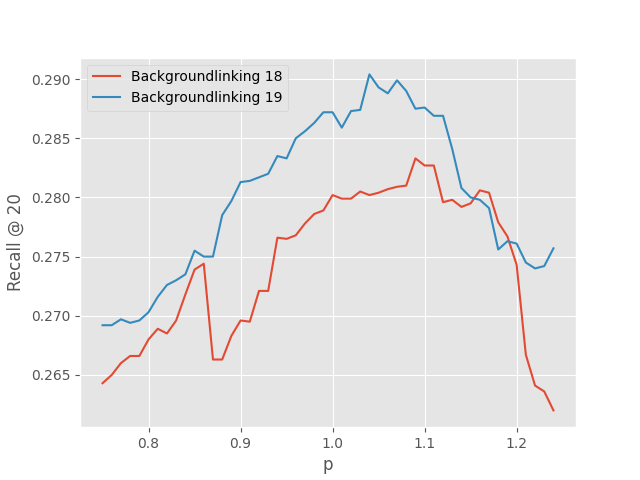
\includegraphics[width=0.9\linewidth]{./imgs/recall-20-geesedb.png}
	\caption{Recall @ 20 for varying levels of $p$}
	\label{geesedb-recall-20}
\end{figure}

\begin{figure}
	\centering
	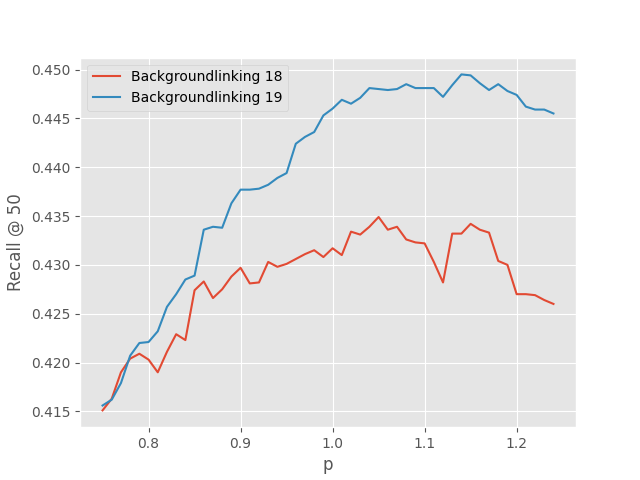
\includegraphics[width=0.9\linewidth]{./imgs/recall-50-geesedb.png}
	\caption{Recall @ 50 for varying levels of $p$}
	\label{geesedb-recall-50}
\end{figure}

\begin{figure}
	\centering
	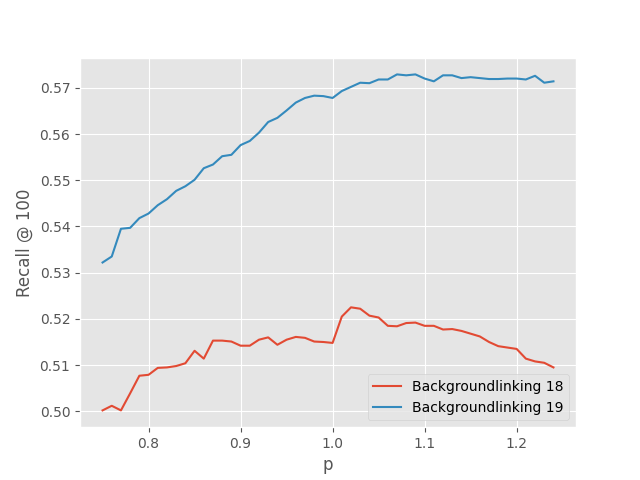
\includegraphics[width=0.9\linewidth]{./imgs/recall-100-geesedb.png}
	\caption{Recall @ 100 for varying levels of $p$}
	\label{geesedb-recall-100}
\end{figure}

\Cref{geesedb-recall-20,geesedb-recall-50,geesedb-recall-100} show the effectiveness scores for values of $p$ from $0.75$ to $1.25$ for recall at 20, 50 and 100. When $p = 1$, documents written by the same author get the same score. Values for $p$ lower than $1$ would decrease the scores for articles written by the same author.  
We see that for both collections, a slight boost of documents that are written by the same author, represented by the values $1 < p < 1.1$, does increase recall at different depths for both document collections.  However when $p$ becomes larger than $1.1$ the recall tends to decrease, especially for recall at depth $20$. 
This experiment shows that it is quite easy to use GeeseDB for retrieval experiments and adding metadata; showing that including metadata might benefit first stage ranking methods.

\section{Conclusion}
This chapter described the prototype implementation of GeeseDB, and how we envision graph databases be used for information retrieval research.
The GeeseDB system can be considered the answer on our research question: \emph{Can we extend the benefits from using relational databases for information retrieval to using graph databases, while being able to express graph-related problems easier?}
As GeeseDB is built on top of a relational engine it automatically inherits the benefits of using relational databases for IR. As GeeseDB can process graph queries, we also are able to express graph related problems. 

GeeseDB is still however a prototype system, and more functionalities need to be implemented. In particular, although the architecture is not coupled, it is not (yet) as efficient as traditional methods that do use coupled architectures. 

Not all graph operators have been supported in the current implementation. In order to make GeeseDB a usable system for IR researchers, more operators need to be implemented and the system needs to be developed to be more robust. 
 

\chapter{Data Modeling using Graphs}
\chapter{Applications}
\chapter{Conclusion}
\bibliographystyle{acm}
\bibliography{./refs.bib}

\backmatter
% bibliography, glossary and index would go here.
\chapter*{Summary}
\addcontentsline{toc}{chapter}{Summary}
\markboth{Summary}{Summary}
\chapter*{Samenvatting}
\addcontentsline{toc}{chapter}{Samenvatting}
\markboth{Samenvatting}{Samenvatting}

Het vinden van relevante informatie in een grote verzameling van documenten is een zeer uitdagende taak, zeker wanneer alleen tekst in overweging wordt genomen bij het bepalen of een document relevant is. Dit onderzoek maakt gebruik van grafen om informatiebehoeften uit te drukken waar meer in overweging genomen moet worden dan alleen tekst. In sommige gevallen gebruiken we, voor de data representatie, in plaats van \emph{inverted indexes}, data management systemen om data op te slaan.

Allereerst, laten we zien dat relationele database systemen geschikt zijn voor \emph{information retrieval} experimenten.
Een door ons gebouwd prototype systeem implementeert een hele reeks verbeteringen aan het BM25-rangschikking algoritme die zijn voorgesteld in de literatuur. In een grootschalig reproductie onderzoek vergelijken we deze verbeteringen en vinden we dat de verschillen in effectiviteit kleiner zijn dan we op grond van de literatuur zouden verwachten. 
We kunnen gemakkelijk wisselen tussen versies van BM25 door de SQL-query slechts weinig te herschrijven met simpele variaties op een onderliggende SQL query. 

Hiermee valideren we het nut van relationele databases voor reproduceerbaar IR-onderzoek.
Vervolgens breiden we het datamodel uit naar een graaf datamodel. Met dit graaf datamodel kunnen we meer diverse gegevens uitdrukken dan alleen tekst. 
We kunnen complexe informatiebehoeften makkelijker uitdrukken met een bijbehorende graaf querytaal, dan wanneer een relationele taal wordt gebruikt. Dit model is gebouwd bovenop een \emph{embedded} database systeem, hierdoor kunnen we data dat geproduceerd wordt door dit systeem snel voor een andere applicatie gebruiken.

Een van de aspecten die we in de graaf vastleggen, is informatie over entiteiten. We gebruiken het Radboud Entity Linking (REL) systeem om entiteit informatie te koppelen aan documenten. Om een grote documentverzameling efficiënt te annoteren met REL hebben we de efficiëntie van REL verbeterd. Na deze verbeteringen hebben we REL gebruikt om annotaties te maken voor de MS MARCO-document- en passage-collecties. Met behulp van deze annotaties kunnen we de \emph{recall} voor moeilijkere MS MARCO-query's aanzienlijk verbeteren. Deze entiteiten worden ook gebruikt voor een interactieve demonstratie waarbij de geografische gegevens van entiteiten worden gebruikt.

\chapter*{Acknowlegements}
\addcontentsline{toc}{chapter}{Acknowlegements}
\markboth{Acknowlegements}{Acknowlegements}
\chapter*{Research Data Management}
\addcontentsline{toc}{chapter}{Research Data Management}
\markboth{Research Data Management}{Research Data Management}
\label{chp:research_data_management}

This thesis research has been carried out under the research data management policy of the Institute for Computing and Information Science of the Radboud University, the Netherlands\footnote{\url{https://www.ru.nl/icis/research-data-management/}}.

The following research datasets have been produced during this PhD research:

\begin{itemize}
	\item Resources for~\cref{ir-using-relational-databases}
	\begin{itemize}
		\item Code for OldDog~\citep{olddog-docker}:
		
		\href{https://doi.org/10.5281/zenodo.7892260}{chriskamphuis/olddog}: (v1.0.0). Zenodo. 10.5281/zenodo.3255060
		
		\item Code for the OldDog docker~\citep{olddog-docker}:
		
		\href{https://doi.org/10.5281/zenodo.3255060}{osirrc/olddog-docker}: (v1.0.0). Zenodo. 10.5281/zenodo.3255060
	\end{itemize}
	
	\item Resources for~\cref{from-tables-to-graphs}
	\begin{itemize}
		\item Code for GeeseDB~\citep{geesedb}:
		
		\href{https://doi.org/10.5281/zenodo.7892326}{informagi/GeeseDB}: (v0.0.2). Zenodo. 10.5281/zenodo.7892326
	\end{itemize}
	
	\item Resources for~\cref{a-graph-of-entities}
	\begin{itemize}
		\item Code for REBL~\citep{rebl}:
		
		\href{https://doi.org/10.5281/zenodo.7892359}{informagi/REBL}: (v0.0.1). Zenodo. 10.5281/zenodo.7892359
	\end{itemize}
	
	\item Resources for~\cref{mmead}
	\begin{itemize}
		\item Code for MMEAD~\citep{mmead}:
		
		\href{https://doi.org/10.5281/zenodo.7897027}{informagi/mmead}: (v0.1.0). Zenodo. 10.5281/zenodo.7897027
		
		\item Data for MMEAD~\citep{mmead}:
		
		\href{https://doi.org/10.5281/zenodo.7896782}{informagi/mmead}: (v0.0.1). Zenodo. 10.5281/zenodo.7896782
	\end{itemize}
	
\end{itemize}
\chapter*{Curriculum Vit\ae}
\addcontentsline{toc}{chapter}{Curriculum Vit\ae}
\markboth{Curriculum Vit\ae}{Curriculum Vit\ae}

\end{document}